
%%%%%%%%%%%%%%%%%%%%%%%%%%%%%%%%%%%%%%%%%%%%%%%%%%%%%%%%%
\section{Kaon candidate selection in the beamline}\label{sec:BeamlineSelection}
\subsection{Overview of the LArIAT Beamline}\label{sec:BeamlineOverview}
%%%%%%%%%%%%%%%%%%%%%%%%%%%%%%%%%%%%%%%%%%%%%%%%%%%%%%%%%
The LArIAT experiment takes place at the Fermilab Test Beam Facility (FTBF) located in the Meson Building at Fermilab. A beam of 120~GeV protons is transported to the Meson Building and split to make two beam lines known as MCenter and MTest. LArIAT is served by the MCenter beam line, whose primary beam of 120~GeV protons impinges upon a thick target (25~cm) to create a secondary beam of charged particles, mainly kaons, 8 - 80 GeV range. This collimated kaon beam is momentum-selected and then transported the MC7 radiation enclosure, the LArIAT experiment hall.  

In the MC7 enclosure the secondary beam focuses onto a thick copper target and the resulting tertiary beam is collimated by a 1~m iron shield with an opening $-13\deg$ to beam's right with respect to the secondary beam direction. Two analyzing dipole magnets steer the beam path $+10\deg$, selecting a momentum window within 0.2 and 2.0~GeV/c and sign-selecting the particles and steering them to the TPC. The tertiary beam is instrumented with a pair of Time-of-Flight (TOF) scintillating detectors,  four Wire Chambers (WC) which allow measurement of each particle's momentum based on the location of the hits in the wire chambers, two Aerogel Cherenkov counters (AG) of different Cherenkov threshold to allow for $\mu / \pi$ separation, the LArTPC detector and a Muon Range Stack. Figure \ref{fig:beamlineschematic} gives a diagram of the tertiary beam line within the MC7 enclosure.

\begin{figure}[htb]
\begin{center}
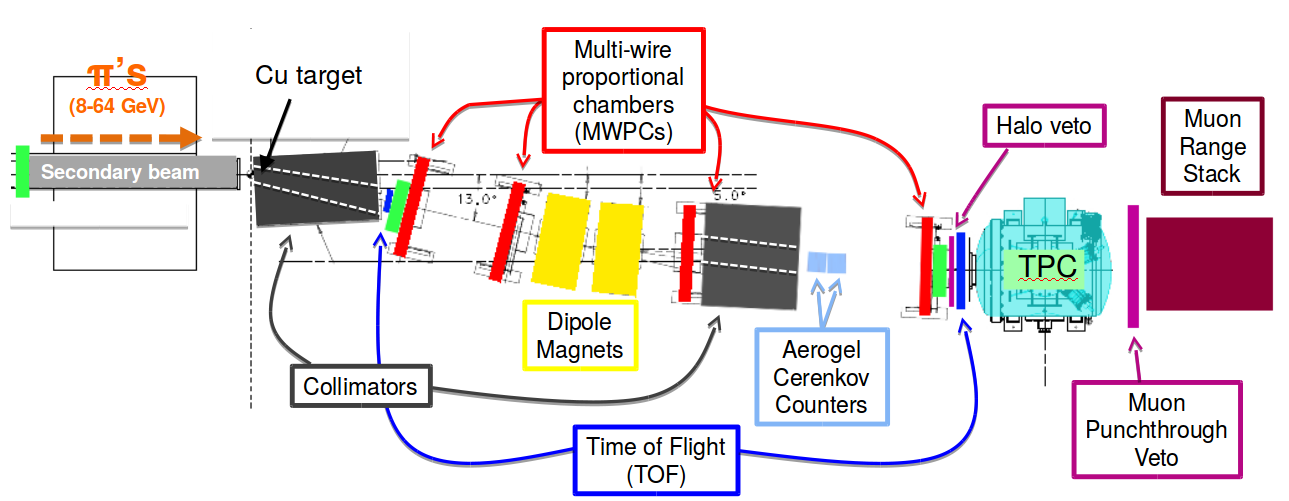
\includegraphics[scale=0.25]{./images/mc7beamline.png}
\end{center}
\caption{Schematic of the Tertiary Beam line within the MC7 enclosure.}
\label{fig:beamlineschematic}
\end{figure}

In this analysis, only the information from the Wire Chambers and the Time-of-Flight is used for particle identification. In particular, it is possible to calculate the mass of a given beamline track using the following equation

\begin{equation}
mass = \frac{p}{c}\sqrt{(\frac{TOF \times c}{l})^2 -1}
\end{equation}
where $p$ represents the measured momentum from the wire chamber, $TOF$ represents the time-of-flight measured as the difference between the two time-of-flight paddles in the LArIAT beamline, $l$ is path length the particle traveled down the beamline, and $c$ represents the speed of light. As is outlined in Section \ref{sec:EventSelection}, this allows us to select events based on the particle species.

%%%%%%%%%%%%%%%%%%%%%%%%%%%%%%%%%%%%%%%%%%%%%%%%%%%%%%%%%%%%%%%%%%%%%%%%%
\subsection{Beam composition}\label{sec:G4BeamlineMC}
%%%%%%%%%%%%%%%%%%%%%%%%%%%%%%%%%%%%%%%%%%%%%%%%%%%%%%%%%%%%%%%%%%%%%%%%%



\subsection{Data Selection Cut}\label{sec:DataSelectionCut}
\subsubsection{Beamline Candidates}\label{sec:BeamlineCandidates}

%%%%%%%%%%%%%%%%%%%%%%%%%%%%%%%%%%%%%%%%%%%%%%%%%%%%%%%%%%%%
For each sample listed in Table \ref{tab:datasamples}, we outline the event selection used to select this data.

\begin{itemize}
\item \textbf{Time Stamp Filter}

A filter is used to select events which occurred in time with the beam. These events typically coincide with the first 6 seconds of the beam spill, and therefore the events are filtered using the following LArIATsoft settings

\begin{verbatim}
tfilt:      @local::lariat_timestampfilter

# ====================================================================
# Specify range of events to select.  For Run I/II:
#   - pedestal events:  ~ 0.  - 1.2 sec
#   - beam events:      ~ 1.2 - 5.5 sec
#   - cosmic events:    ~ > 5.5 sec
#   (default selects ALL events)
physics.filters.tfilt.T1:                       1.2
physics.filters.tfilt.T2:                       5.5
physics.filters.tfilt.RequireRawDigits:         true

\end{verbatim}



\item \textbf{Beamline Reconstruction}

The standard LArIAT beamline reconstruction is used to select events which have a wire chamber track and TOF information in an individual event using the following modules.
\begin{verbatim}
### beamline elements ###

wctrack:     @local::lariat_wctrackbuilder
tof:         @local::lariat_tof
agcounter:   @local::lariat_aerogel
\end{verbatim}


\textbf{For Run-I we use these default parameters:}
\begin{verbatim} 
physics.producers.wctrack.PickyTracks:                          false
physics.producers.tof.HitThreshold:                           -10.0  
physics.producers.tof.HitDiffMeanUS:                            0.6  
physics.producers.tof.HitDiffMeanDS:                            1.0  
physics.producers.tof.HitMatchThresholdUS:                      3.0  
physics.producers.tof.HitMatchThresholdDS:                      6.0  
physics.producers.tof.HitWait:                                  20.
\end{verbatim}

\textbf{For Run-II we use these default parameters:}
\begin{verbatim} 
physics.producers.wctrack.PickyTracks:                          false
physics.producers.tof.HitThreshold:                             -3.
physics.producers.tof.HitDiffMeanUS:                            0.5  
physics.producers.tof.HitDiffMeanDS:                            0.4  
physics.producers.tof.HitMatchThresholdUS:                      3.0  
physics.producers.tof.HitMatchThresholdDS:                      6.0  
physics.producers.tof.HitWait:                                  20.
\end{verbatim}

We require the tracks reconstructed in the wire chamber satisfy the criteria known as a ``picky track''. ``Picky tracks'' correspond to tracks reconstructed using hits in all four wire chambers. In these events, one and only one hit in each wire chamber track can be reconstructed per event and the track satisfies a straightness requirement in the Y-Z plane. These tracks have more accurate measure of the particle momentum than the ``high yield'' (HY) tracks.  HY tracks only require hits in three out of four of the wire chamber tracks and can have multiple wire chamber hits reconstructed per event. HY tracks yield better statistics: a subset of HY tracks can be used as a orthogonal sample for the study of systematics. Details about wire chamber track reconstruction can be found in \cite{WCTrackReco}

\item \textbf{Particle Mass Filtering}
Using the beamline reconstruction, it is possible to calculate the mass of a given track, as shown in Figure \ref{fig:mass}. The classification of events into the different samples follows:

\begin{itemize}
\item \underline{$\pi, \mu, e$:} 0~MeV $<$ mass $<$ 350~MeV

\item \underline{kaon:} 350~MeV $<$ mass $<$ 650~MeV

\item \underline{proton:} 650~MeV $<$ mass $<$ 3000~MeV

\end{itemize}

\begin{figure}[htb]
\centering
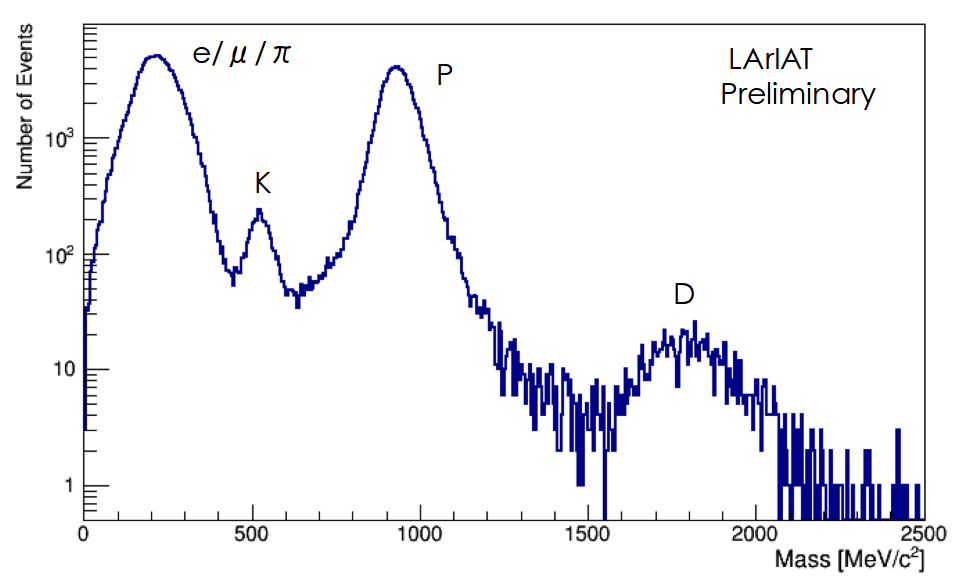
\includegraphics[width=0.70\textwidth]{images/mass.png}
\caption{The mass plotted for a sample of Run-II events reconstructed in the beamline. The classification of the events into $\pi, \mu, e$, kaon, or proton is based on this distribution.}
\label{fig:mass}
\end{figure}

For this analysis we require 350~MeV $<$ mass $<$ 650~MeV to select a sample of $K$ candidates for further event selection. The full event reduction table for these cuts is presented in Section \ref{sec:Results}.

\end{itemize}


\subsubsection{Candidates}\label{sec:Candidates}
\subsubsection{Contamination from different particle species in the beam line }\label{sec:Contamination}
\section{Kaon Analysis} \label{sec:kaonAnalysis} 
\section{Systematics} \label{sec:Systematics} 
\section{Results}\label{sec:Results}
